\documentclass[tikz,border=2mm]{standalone}
\usetikzlibrary{positioning,fit,arrows.meta,calc}
\begin{document}
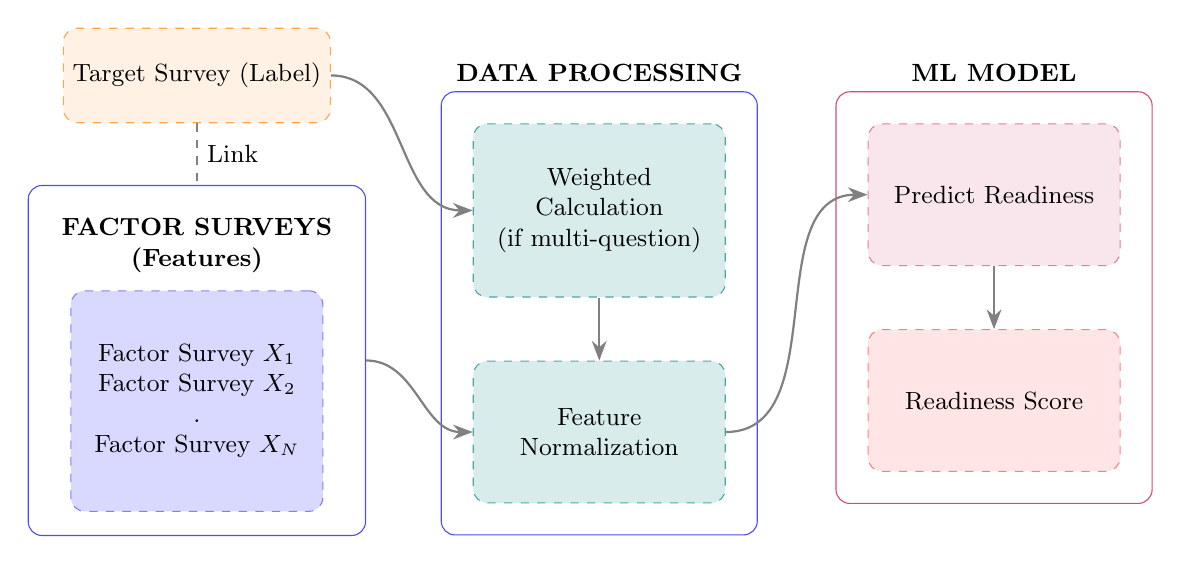
\begin{tikzpicture}[
  box/.style={draw,dashed,rounded corners=5pt,align=center,font=\small},
  container/.style={draw,rounded corners=5pt,inner sep=4mm},
  arr/.style={gray,thick,-{Stealth[length=2.5mm]}}
]
% Left column - Target Survey
\node[box,draw=orange!70,fill=orange!10,minimum width=32mm,minimum height=12mm] (target) {Target Survey (Label)};

% Middle column - Data Processing
\node[box,draw=teal!70,fill=teal!15,minimum width=32mm,minimum height=22mm,right=18mm of target.south east,anchor=north west] (weighted) {Weighted\\Calculation\\(if multi-question)};
\node[box,draw=teal!70,fill=teal!15,minimum width=32mm,minimum height=18mm,below=8mm of weighted] (normalize) {Feature\\Normalization};
\node[container,draw=blue!70,fit=(weighted)(normalize),label={[font=\small\bfseries]above:DATA PROCESSING}] (dbox) {};

% Left column - Factor Surveys (aligned to dbox bottom)
\node[box,draw=blue!50,fill=blue!15,minimum width=32mm,minimum height=28mm,anchor=south] at ([yshift=3mm]target.south|-dbox.south) (factors) {Factor Survey $X_1$\\Factor Survey $X_2$\\.\\Factor Survey $X_N$};
\node[font=\small\bfseries,align=center,above=1mm of factors] (flabel) {FACTOR SURVEYS\\(Features)};
\node[container,draw=blue!70,inner sep=3mm,fit=(factors)(flabel)] (fbox) {};

% Link between target and factor surveys
\draw[gray,dashed,thick] (target.south) -- node[right,font=\small,black]{Link} (fbox.north);

% Right column - ML Model
\node[box,draw=purple!50,fill=purple!10,minimum width=32mm,minimum height=18mm,right=18mm of weighted.north east,anchor=north west] (predict) {Predict Readiness};
\node[box,draw=red!50,fill=red!10,minimum width=32mm,minimum height=18mm,below=8mm of predict] (score) {Readiness Score};
\node[container,draw=purple!70,fit=(predict)(score),label={[font=\small\bfseries]above:ML MODEL}] (mbox) {};

% Arrows
\draw[arr] (target.east) to[out=0,in=180] (weighted.west);
\draw[arr] (fbox.east) to[out=0,in=180] (normalize.west);
\draw[arr] (weighted.south) -- (normalize.north);
\draw[arr] (normalize.east) to[out=0,in=180] (predict.west);
\draw[arr] (predict.south) -- (score.north);
\end{tikzpicture}
\end{document}